\documentclass[aspectratio=1610,handout=false]{beamer}
\usepackage{beamer-s4ndm4n}
\usepackage{kantlipsum} % blind text
\graphicspath{{gfx/}} % to shorten \includegraphics

\title{Example Slide Deck Featuring s4ndm4n Dark Theme}
\subtitle{To Be Used With \LaTeX{} \texttt{beamer}}
\author{\href{https://github.com/ruempel}{Andreas Rümpel}}
\institute{\href{https://github.com/ruempel/beamer-s4ndm4n}{https://github.com/ruempel/beamer-s4ndm4n}}
\date[2017-12-09]{9 December 2017}

\begin{document}
\maketitle

\begin{frame}
	\frametitle{Standard Elements}
	\framesubtitle{Optional Frame Subtitle}
	\begin{block}{Box Created from \texttt{block} with Some Content}
		This \texttt{block} features a nested item list.
		\begin{itemize}
			\item first item
			\item second item
			\begin{itemize}
				\item first nested item
				\item second nested item
			\end{itemize}
		\end{itemize}
	\end{block}
\end{frame}


\begin{frame}
	\frametitle{Another Frame with Multiple Boxes}
	\begin{block}{First Box with Text}
		\kant[9]
	\end{block}
	
	\begin{block}{Second Box with Enumeration}
		\begin{enumerate}
			\item first item with \alert{alerted text}
			\item second item
			\item third item
		\end{enumerate}
		\end{block}
\end{frame}


\begin{frame}
	\frametitle{Gingerbread House}
	\centering
	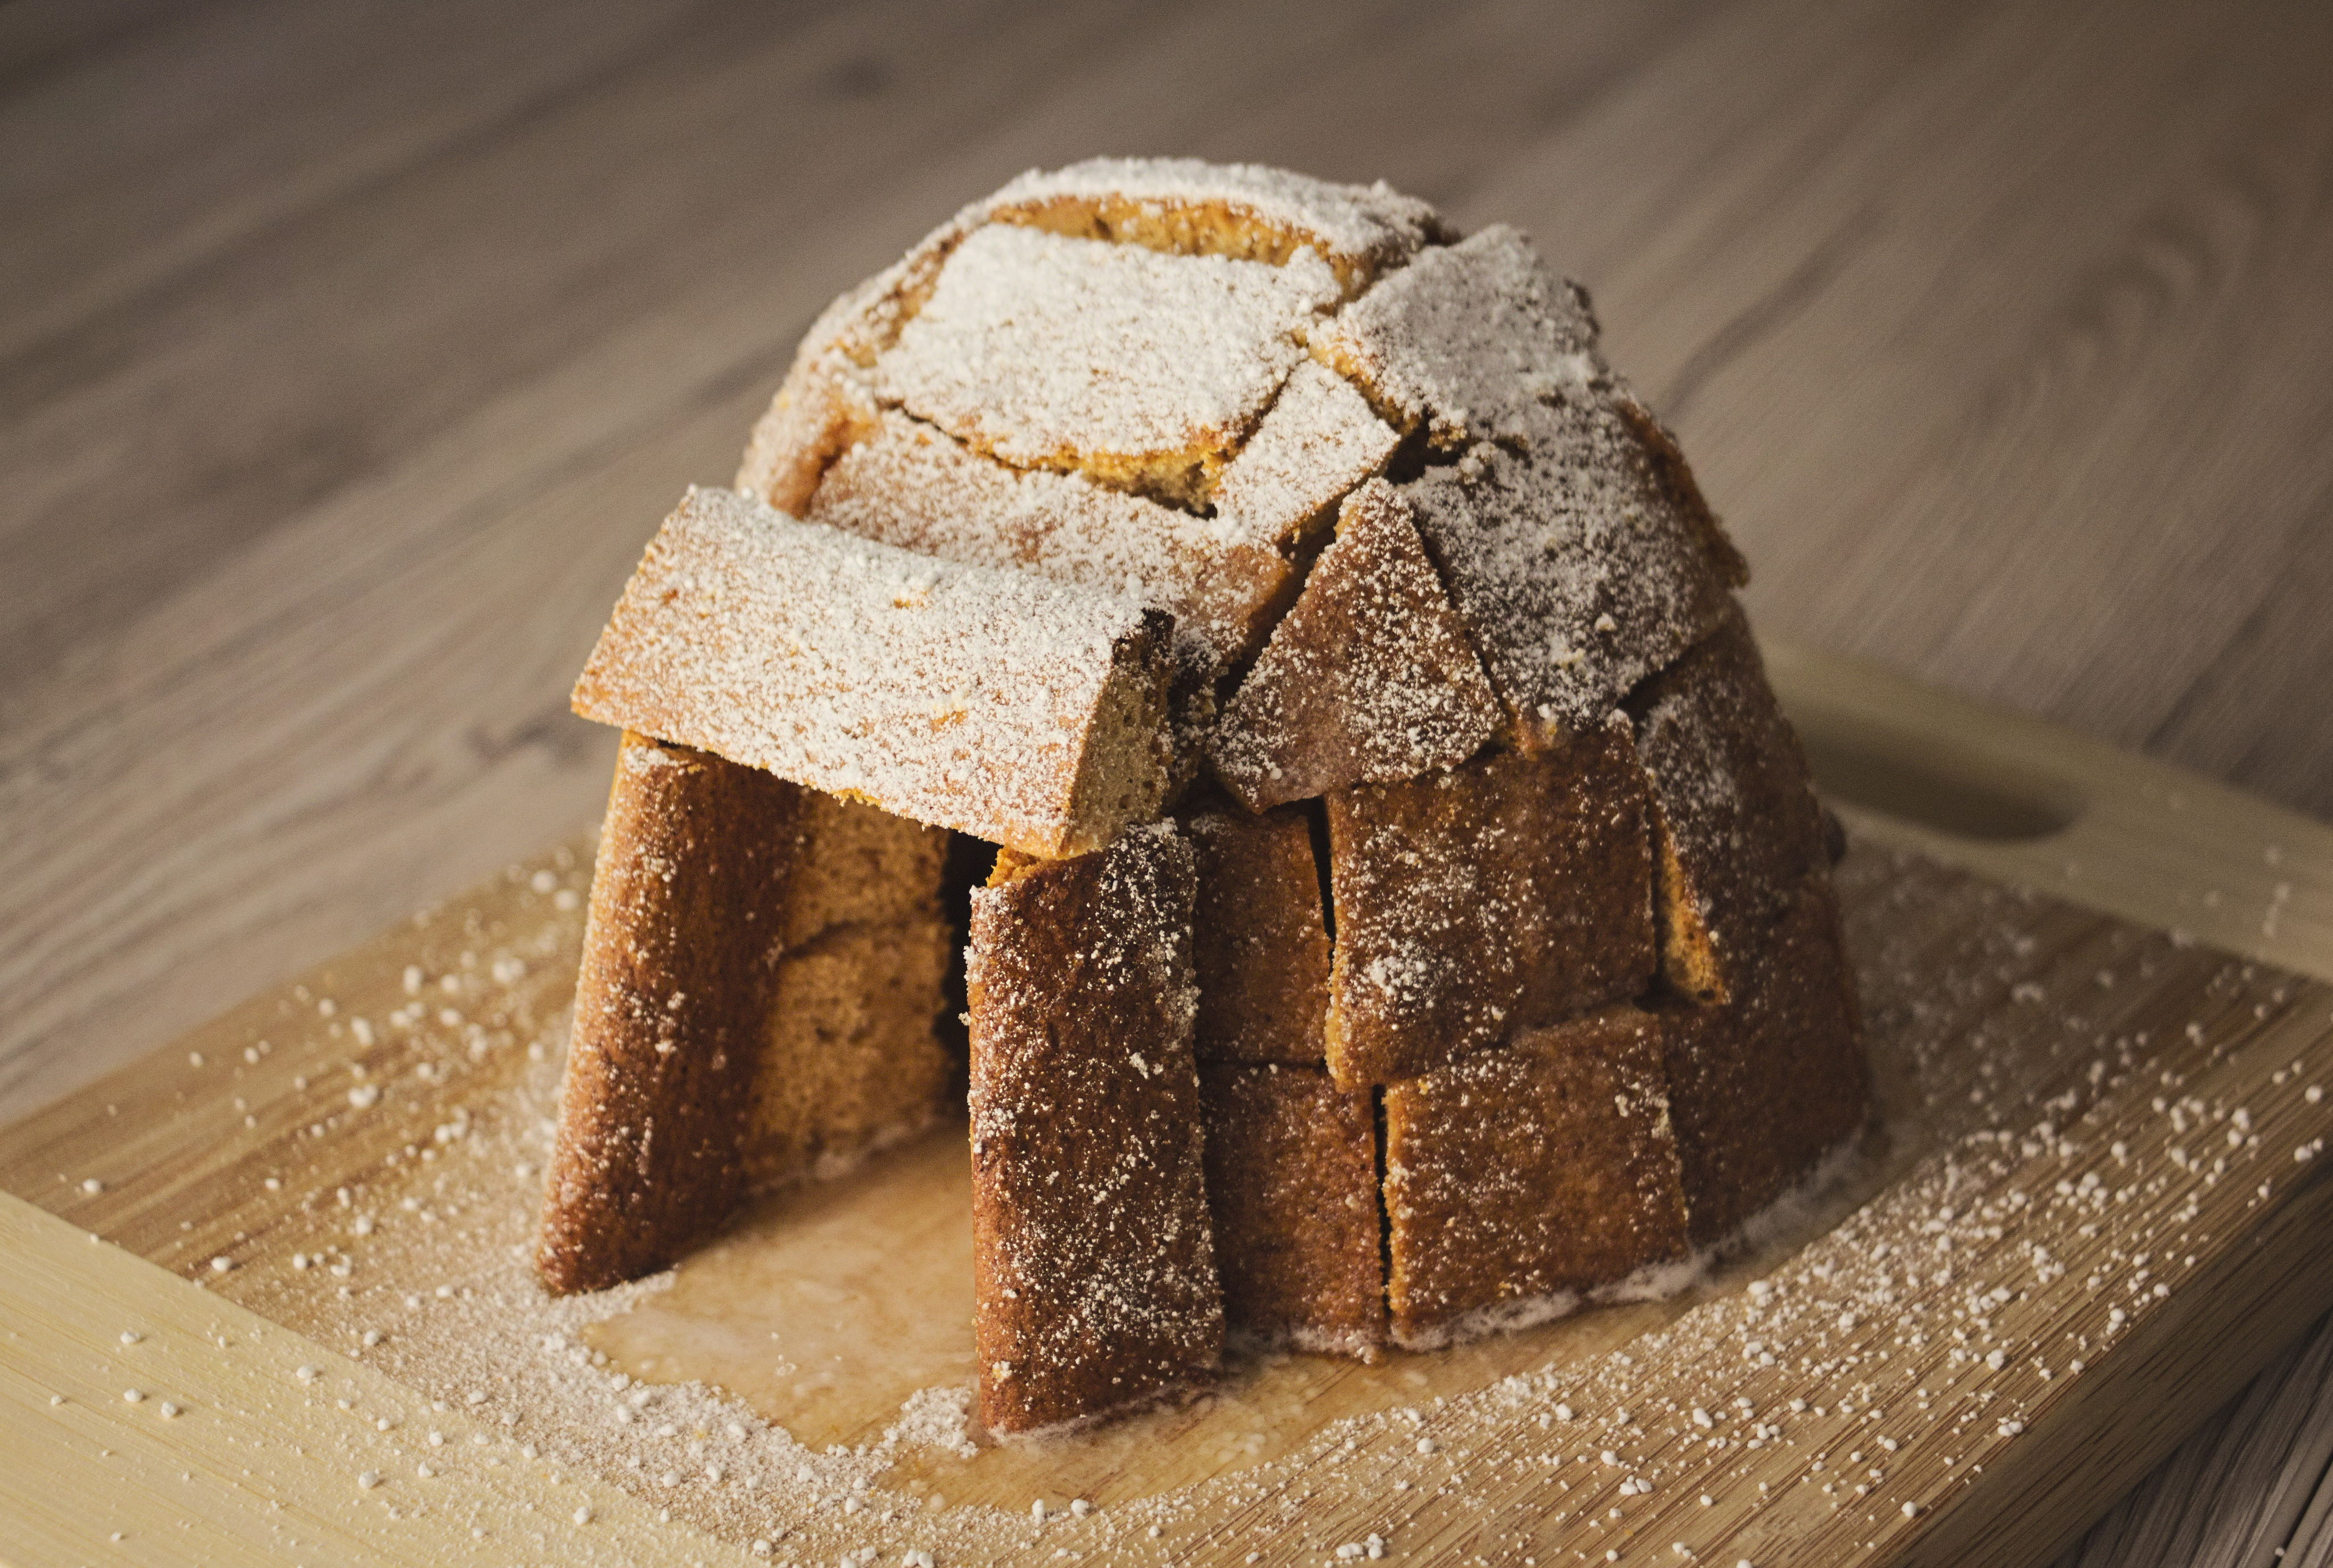
\includegraphics[width=0.8\textwidth]{gingerbread-house}
\end{frame}
\end{document}